% ------------------------------------------------------------------
% Orynth v2 — End-to-end system, bench to swarm.
% Multi-page reference: UML diagrams, network topology, sequence flows,
% and field setup. Compiles standalone — no external images required.
% Drop JPGs into ./images/ and uncomment the matching \includegraphics
% line to replace any photo placeholder.
%
% Build:   pdflatex -interaction=nonstopmode end_to_end_setup.tex
% Twice  for cross-references; output: end_to_end_setup.pdf
% ------------------------------------------------------------------
\documentclass[11pt,a4paper]{article}

\usepackage[a4paper, margin=2cm, top=2.4cm, bottom=2.4cm]{geometry}
\usepackage{graphicx}
\usepackage{tikz}
\usetikzlibrary{shapes, shapes.geometric, shapes.symbols, shapes.multipart,
                arrows.meta, positioning, fit, backgrounds, calc,
                shadows.blur, decorations.pathreplacing, patterns}
% pgf-umlsd would be nicer but the version shipped with TeX Live 2023 has
% scaling bugs; sequence diagrams below are written in plain TikZ instead.
\usepackage{xcolor}
\usepackage{titlesec}
\usepackage[hidelinks]{hyperref}
\usepackage{enumitem}
\usepackage{caption}
\usepackage{tabularx}
\usepackage{array}
\usepackage{booktabs}
\usepackage{fancyhdr}
\usepackage{lmodern}
\usepackage{microtype}
\usepackage{titling}
\usepackage{tcolorbox}
\tcbuselibrary{skins, breakable}

% --- Brand colors ---
\definecolor{fcblue}{HTML}{1f4e79}
\definecolor{rcorange}{HTML}{c75500}
\definecolor{jetsonteal}{HTML}{2e7d7d}
\definecolor{gcspurple}{HTML}{5a3370}
\definecolor{accentgreen}{HTML}{2e7d32}
\definecolor{bggrey}{HTML}{f4f4f4}
\definecolor{linegrey}{HTML}{555555}
\definecolor{lightaccent}{HTML}{e8eef5}
\definecolor{warnred}{HTML}{b3261e}

% --- TikZ box styles ---
\tikzset{
  hwbox/.style={rectangle, draw=fcblue, fill=fcblue!8, very thick,
                rounded corners=3pt, minimum width=3.2cm, minimum height=1.2cm,
                align=center, font=\small},
  rcbox/.style={rectangle, draw=rcorange, fill=rcorange!10, very thick,
                rounded corners=3pt, minimum width=3.2cm, minimum height=1.2cm,
                align=center, font=\small},
  jetbox/.style={rectangle, draw=jetsonteal, fill=jetsonteal!10, very thick,
                 rounded corners=3pt, minimum width=3.2cm, minimum height=1.2cm,
                 align=center, font=\small},
  gcsbox/.style={rectangle, draw=gcspurple, fill=gcspurple!10, very thick,
                 rounded corners=3pt, minimum width=3.2cm, minimum height=1.2cm,
                 align=center, font=\small},
  fcbox/.style={rectangle, draw=fcblue, fill=fcblue!15, very thick,
                minimum width=3cm, minimum height=1.4cm,
                align=center, font=\small\bfseries},
  swcomp/.style={rectangle, draw=jetsonteal, fill=jetsonteal!8, thick,
                 minimum width=3.6cm, minimum height=1.1cm, align=center, font=\small},
  drone/.style={rectangle, draw=fcblue, fill=lightaccent, very thick,
                rounded corners=4pt, minimum width=2.1cm, minimum height=1.5cm,
                align=center, font=\scriptsize, drop shadow},
  ddsnode/.style={circle, draw=accentgreen, fill=accentgreen!10, thick,
                  minimum size=0.5cm, inner sep=0},
  link/.style={->, very thick, >={Stealth[length=3mm,width=2mm]}, draw=linegrey},
  biglink/.style={<->, very thick, >={Stealth[length=3mm,width=2mm]}, draw=linegrey},
  faintlink/.style={->, thick, >={Stealth[length=2.5mm,width=1.7mm]}, draw=linegrey!70, dashed},
  linklabel/.style={font=\scriptsize\itshape, fill=white, inner sep=2pt},
  % --- sequence diagram styles ---
  sdactor/.style={draw=fcblue, very thick, fill=fcblue!10, font=\small\bfseries,
                  minimum width=3cm, minimum height=0.7cm, rounded corners=2pt, align=center},
  sdactorlight/.style={draw=jetsonteal, very thick, fill=jetsonteal!10, font=\small\bfseries,
                       minimum width=3cm, minimum height=0.7cm, rounded corners=2pt, align=center},
  sdactorops/.style={draw=gcspurple, very thick, fill=gcspurple!10, font=\small\bfseries,
                     minimum width=3cm, minimum height=0.7cm, rounded corners=2pt, align=center},
  lifeline/.style={dashed, draw=linegrey!60, thick},
  sdmsg/.style={->, very thick, >={Stealth[length=2.8mm,width=1.8mm]}, draw=linegrey},
  sdret/.style={->, thick, dashed, >={Stealth[length=2.5mm,width=1.5mm]}, draw=linegrey!80},
  sdself/.style={->, thick, >={Stealth[length=2mm,width=1.4mm]}, draw=linegrey},
  sdlab/.style={font=\scriptsize\ttfamily, fill=white, inner sep=2pt},
  sdlabit/.style={font=\scriptsize\itshape, fill=white, inner sep=2pt},
  notebox/.style={draw=warnred!70, fill=warnred!8, rounded corners=2pt,
                  font=\scriptsize\itshape, inner sep=4pt, align=center},
  activation/.style={draw=fcblue, fill=lightaccent, very thick},
}

% --- Photo placeholder ---
% #1 width in cm, #2 height in cm, #3 caption describing the shot to take.
\newcommand{\photoplaceholder}[3]{%
  \begin{center}
  \begin{tikzpicture}
    \node[draw=gray!60, line width=1pt, fill=bggrey,
          minimum width=#1 cm, minimum height=#2 cm,
          inner sep=0, align=center] (ph) {};
    \draw[draw=gray!35, dashed] (ph.south west) -- (ph.north east);
    \draw[draw=gray!35, dashed] (ph.south east) -- (ph.north west);
    \node[anchor=north, font=\small\itshape\color{gray!75}]
      at ([yshift=-0.45cm]ph.north) {[ photo placeholder ]};
    \node[anchor=south, font=\scriptsize\color{gray!75}, align=center,
          text width={#1 cm - 1cm}] at ([yshift=0.45cm]ph.south) {#3};
  \end{tikzpicture}
  \end{center}
}

% --- Title block ---
\title{\bfseries Orynth v2 \\ \Large End-to-End System: from Bench to Swarm}
\author{\large Architecture reference --- diagrams, sequences, field setup}
\date{Revision: \today}

% --- Section style ---
\titleformat{\section}{\Large\bfseries\color{fcblue}}{\thesection.}{0.6em}{}
\titlespacing*{\section}{0pt}{0.4em}{0.6em}
\titleformat{\subsection}{\large\bfseries\color{jetsonteal}}{\thesubsection.}{0.5em}{}

% --- Header/footer ---
\pagestyle{fancy}
\fancyhf{}
\fancyfoot[C]{\small\thepage}
\fancyhead[L]{\small\itshape Orynth v2 --- End-to-End Setup}
\fancyhead[R]{\small\itshape Bench $\rightarrow$ Swarm}
\renewcommand{\headrulewidth}{0.3pt}

\begin{document}

% =================================================================
% TITLE PAGE
% =================================================================
\thispagestyle{empty}
\begin{tikzpicture}[remember picture, overlay]
  \fill[fcblue] (current page.north west) rectangle ([yshift=-3.5cm]current page.north east);
  \node[anchor=north west, text=white, font=\Huge\bfseries]
    at ([xshift=2cm,yshift=-1.2cm]current page.north west) {Orynth v2};
  \node[anchor=north west, text=white, font=\Large]
    at ([xshift=2cm,yshift=-2.4cm]current page.north west)
    {End-to-End System: from Bench to Swarm};
\end{tikzpicture}

\vspace{5.5cm}

\begin{center}
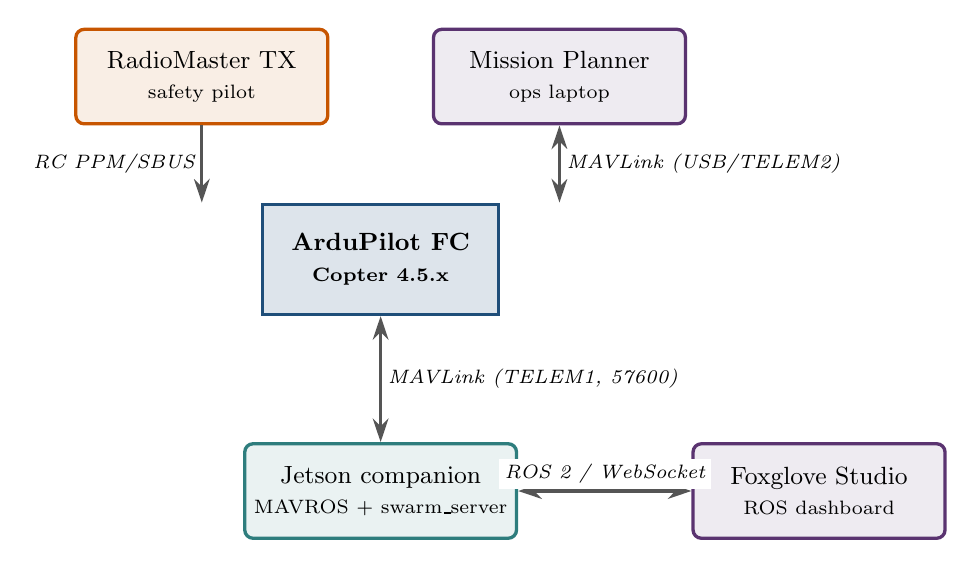
\begin{tikzpicture}[node distance=1.3cm]
  \node[rcbox]    (rc)   {RadioMaster TX\\\scriptsize safety pilot};
  \node[gcsbox, right=of rc]  (mp)   {Mission Planner\\\scriptsize ops laptop};
  \node[fcbox, below=1.6cm of $(rc)!0.5!(mp)$]   (fc)   {ArduPilot FC\\\scriptsize Copter 4.5.x};
  \node[jetbox, below=1.6cm of fc] (jet) {Jetson companion\\\scriptsize MAVROS + swarm\_server};
  \node[gcsbox, right=2.2cm of jet] (fx) {Foxglove Studio\\\scriptsize ROS dashboard};

  \draw[link] (rc.south) -- node[linklabel, left]{RC PPM/SBUS} (rc.south |- fc.north);
  \draw[biglink] (mp.south) -- node[linklabel, right]{MAVLink (USB/TELEM2)} (mp.south |- fc.north);
  \draw[biglink] (fc.south) -- node[linklabel, right]{MAVLink (TELEM1, 57600)} (jet.north);
  \draw[biglink] (jet.east) -- node[linklabel, above]{ROS 2 / WebSocket} (fx.west);
\end{tikzpicture}
\end{center}

\vspace{2.5cm}

\begin{center}
\begin{tcolorbox}[colback=lightaccent, colframe=fcblue, width=0.85\textwidth,
                  arc=2pt, boxrule=0.8pt]
\centering
\textbf{The single idea that makes the rest of this document make sense:}\\[0.4em]
The \textbf{ArduPilot firmware} on the flight controller is the only thing actually flying the drone.
Mission Planner, your RadioMaster TX, and the Jetson companion are all
\emph{clients} talking to that firmware over MAVLink or RC.
This document shows how those clients connect, what each does, and how the same
architecture scales from one drone on a bench to five drones in formation.
\end{tcolorbox}
\end{center}

\vfill
\begin{center}
\small Reference document --- diagrams compile from source; photos are placeholders to be filled.\\
Rebuild: \texttt{pdflatex end\_to\_end\_setup.tex} (twice for cross-refs).\\
\today
\end{center}

\newpage

% =================================================================
% TOC
% =================================================================
\tableofcontents
\newpage

% =================================================================
% §1 — The big picture
% =================================================================
\section{The big picture: three channels, one firmware}

ArduPilot Copter is a multi-client autopilot. Three independent input
channels can address the same firmware simultaneously without conflict;
each has a fixed role, and the firmware enforces a strict priority
when they disagree (\S\ref{sec:authority}).

\vspace{0.6em}
\begin{center}
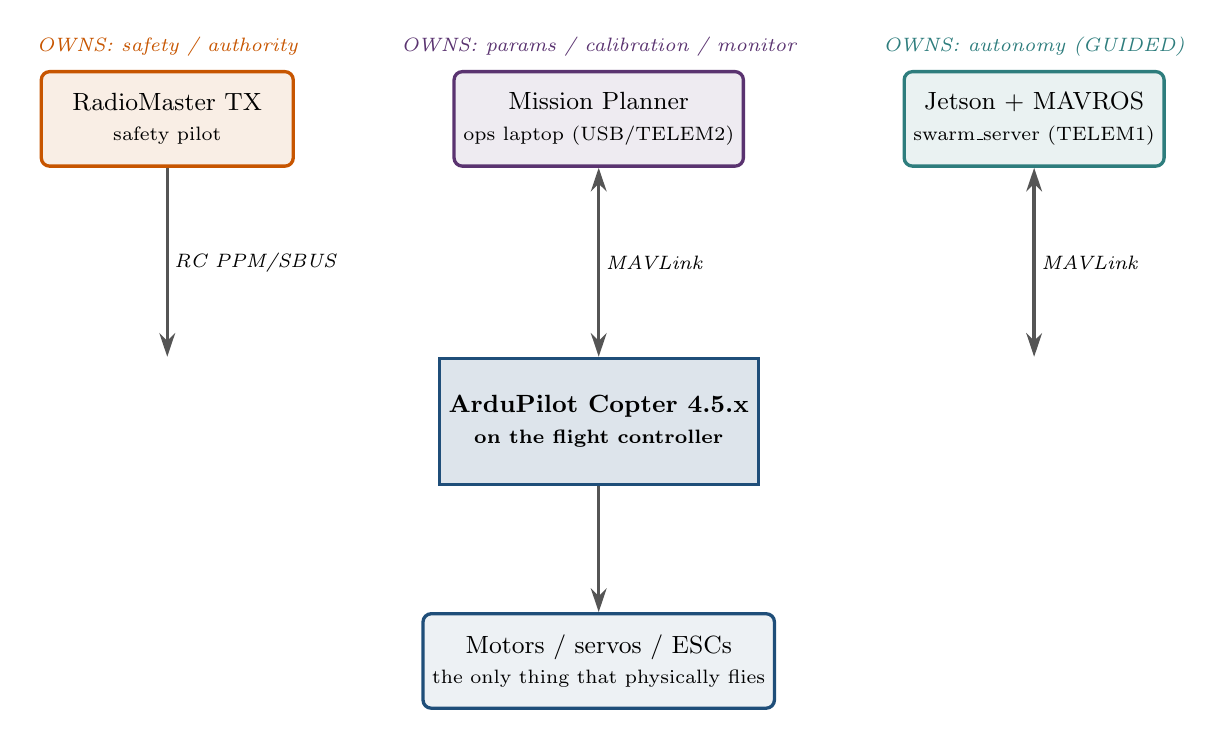
\begin{tikzpicture}[node distance=1.4cm and 1.8cm]
  % Three inputs across the top
  \node[rcbox]                       (rc)  {RadioMaster TX\\\scriptsize safety pilot};
  \node[gcsbox, right=2.0cm of rc]   (mp)  {Mission Planner\\\scriptsize ops laptop (USB/TELEM2)};
  \node[jetbox, right=2.0cm of mp]   (jet) {Jetson + MAVROS\\\scriptsize swarm\_server (TELEM1)};

  % FC in the middle
  \node[fcbox, below=2.4cm of mp, minimum width=4cm, minimum height=1.6cm]
                                      (fc)  {ArduPilot Copter 4.5.x\\\scriptsize on the flight controller};

  % Outputs from FC
  \node[hwbox, below=1.6cm of fc, minimum width=4cm] (act) {Motors / servos / ESCs\\\scriptsize the only thing that physically flies};

  % Links
  \draw[link] (rc.south)  -- node[linklabel, right, pos=0.5]{RC PPM/SBUS} (rc.south  |- fc.north);
  \draw[biglink] (mp.south)  -- node[linklabel, right, pos=0.5]{MAVLink} (mp.south  |- fc.north);
  \draw[biglink] (jet.south) -- node[linklabel, right, pos=0.5]{MAVLink} (jet.south |- fc.north);
  \draw[link, very thick] (fc.south) -- (act.north);

  % Owner labels
  \node[font=\scriptsize\itshape, text=rcorange, anchor=south]
    at ([yshift=0.05cm]rc.north) {OWNS: safety / authority};
  \node[font=\scriptsize\itshape, text=gcspurple, anchor=south]
    at ([yshift=0.05cm]mp.north) {OWNS: params / calibration / monitor};
  \node[font=\scriptsize\itshape, text=jetsonteal, anchor=south]
    at ([yshift=0.05cm]jet.north) {OWNS: autonomy (GUIDED)};

\end{tikzpicture}
\end{center}

\vspace{0.8em}

\begin{tcolorbox}[colback=bggrey, colframe=linegrey!50, arc=2pt, boxrule=0.4pt,
                  title={\small\bfseries What this means for your current bench setup}, fonttitle=\color{fcblue}]
You already have the orange and purple channels. The Jetson + MAVROS layer is
\emph{added in parallel}, on a different serial port (\texttt{TELEM1}).
Nothing about your current RadioMaster + Mission Planner flow changes.
RC override always wins; you can always take a drone manually at any instant.
\end{tcolorbox}

\newpage

% =================================================================
% §2 — Single-drone hardware
% =================================================================
\section{Hardware: a single drone on the bench}

UML deployment view of one drone as it will be wired for Phase~2.5b.
The flight controller is the central node; everything else attaches to it
over a well-defined physical link.

\vspace{0.6em}
\begin{center}
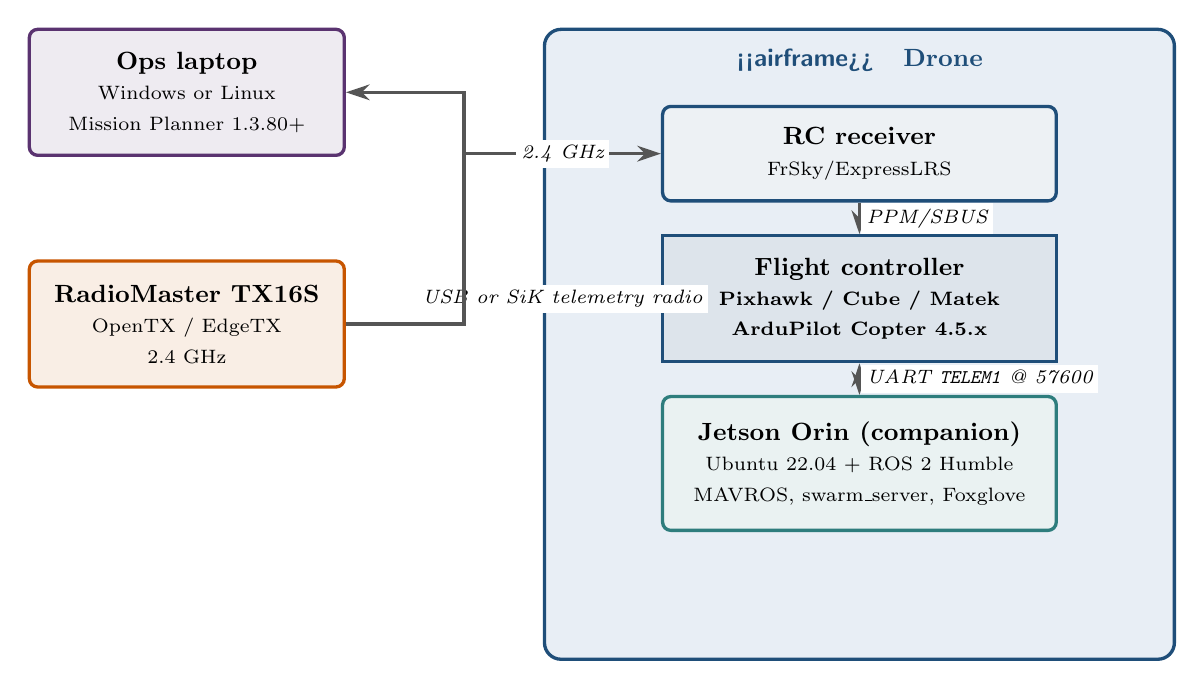
\begin{tikzpicture}[node distance=0.8cm]

  % --- left column: external operator equipment ---
  \node[gcsbox, minimum width=4cm, minimum height=1.6cm] (mplaptop)
       {\textbf{Ops laptop}\\\scriptsize Windows or Linux\\\scriptsize Mission Planner 1.3.80+};
  \node[rcbox, below=1.3cm of mplaptop, minimum width=4cm, minimum height=1.6cm] (radio)
       {\textbf{RadioMaster TX16S}\\\scriptsize OpenTX / EdgeTX\\\scriptsize 2.4 GHz};

  % --- right side: the airframe (drone) as a UML node ---
  \begin{scope}[on background layer]
    \node[draw=fcblue, very thick, fill=lightaccent, rounded corners=6pt,
          minimum width=8cm, minimum height=8cm, anchor=north west] (airframe)
          at ([xshift=2.5cm]mplaptop.north east) {};
  \end{scope}
  \node[anchor=north, font=\small\bfseries\color{fcblue}]
    at ([yshift=-0.15cm]airframe.north) {\textsf{<<airframe>>}\quad Drone};

  % Components inside the airframe
  \node[hwbox, minimum width=5cm, minimum height=1.2cm] (rx)
       at ([yshift=-1.6cm]airframe.north) {\textbf{RC receiver}\\\scriptsize FrSky/ExpressLRS};
  \node[fcbox, below=0.4cm of rx, minimum width=5cm, minimum height=1.6cm] (fc)
       {Flight controller\\\scriptsize Pixhawk / Cube / Matek\\\scriptsize ArduPilot Copter 4.5.x};
  \node[jetbox, below=0.4cm of fc, minimum width=5cm, minimum height=1.7cm] (jetson)
       {\textbf{Jetson Orin (companion)}\\\scriptsize Ubuntu 22.04 + ROS 2 Humble\\\scriptsize MAVROS, swarm\_server, Foxglove};

  % Links
  \draw[biglink] (mplaptop.east) -- ++(1.5,0) |- node[linklabel, near end]{USB or SiK telemetry radio} (fc.west);
  \draw[link]    (radio.east) -- ++(1.5,0) |- node[linklabel, near end]{2.4 GHz} (rx.west);
  \draw[link]    (rx.south) -- node[linklabel, right]{PPM/SBUS} (fc.north);
  \draw[biglink] (fc.south) -- node[linklabel, right]{UART \texttt{TELEM1} @ 57600} (jetson.north);

\end{tikzpicture}
\end{center}

\vspace{0.6em}

\begin{center}
\small
\begin{tabularx}{0.95\textwidth}{@{}lll X@{}}
\toprule
\textbf{Link} & \textbf{Port} & \textbf{Baud / type} & \textbf{Carries} \\
\midrule
Mission Planner $\leftrightarrow$ FC & USB or \texttt{TELEM2}        & 57600--921600    & MAVLink: params, mode, mission, monitoring \\
RadioMaster TX $\to$ RX $\to$ FC     & RC input pins                 & PPM or SBUS      & Stick channels, mode switch (LOITER/POSHOLD/GUIDED) \\
Jetson $\leftrightarrow$ FC          & \texttt{TELEM1} UART          & 57600            & MAVLink: state, setpoints, arming, missions \\
Jetson $\leftrightarrow$ Operator    & WiFi (Foxglove WS \texttt{:8765}) & TCP/IP        & ROS 2 telemetry, services, status \\
\bottomrule
\end{tabularx}
\end{center}

\vspace{0.8em}

\photoplaceholder{15}{6.2}{Suggested shot: the airframe on a stand with the FC visible,
the RC receiver taped/zip-tied, the Jetson cabled into \texttt{TELEM1}, and the
USB cable running to a laptop with Mission Planner open in the background.
Drop the JPG into \texttt{images/bench\_single\_drone.jpg} and uncomment the
\textbackslash{}includegraphics line in the source to replace this placeholder.}

\newpage

% =================================================================
% §3 — Internal software components (UML component diagram)
% =================================================================
\section{Software on the companion: UML component view}

What runs on the Jetson, and how the pieces talk. UML component
diagram with ``provided'' (lollipop) and ``required'' (socket)
interfaces.

\vspace{0.4em}
\begin{center}
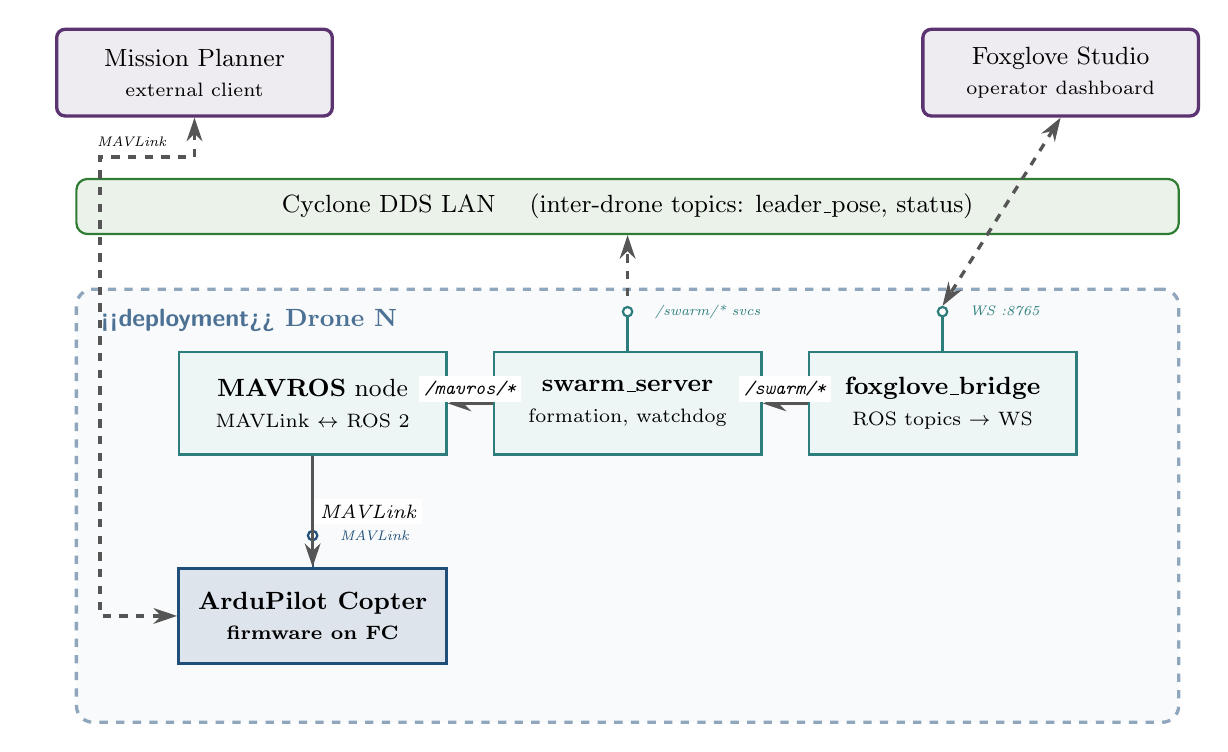
\begin{tikzpicture}[x=1cm, y=1cm]

  % --- External clients (top row) ---
  \node[gcsbox, minimum width=3.5cm, minimum height=1.1cm] (mpc) at (1.5, 8.5)
        {Mission Planner\\\scriptsize external client};
  \node[gcsbox, minimum width=3.5cm, minimum height=1.1cm] (fop) at (12.5, 8.5)
        {Foxglove Studio\\\scriptsize operator dashboard};

  % --- DDS bus ---
  \node[draw=accentgreen, fill=accentgreen!10, thick, rounded corners=4pt,
        minimum width=14cm, minimum height=0.7cm, font=\small] (dds) at (7, 6.8)
        {Cyclone DDS LAN \quad (inter-drone topics: leader\_pose, status)};

  % --- Drone N container ---
  \begin{scope}[on background layer]
    \node[draw=fcblue!50, dashed, fill=fcblue!3, very thick, rounded corners=6pt,
          minimum width=14cm, minimum height=5.5cm] (host) at (7, 3.0) {};
  \end{scope}
  \node[anchor=north west, font=\small\bfseries\color{fcblue!80}]
    at ([xshift=0.2cm, yshift=-0.15cm]host.north west) {\textsf{<<deployment>>}\ Drone N};

  % --- Software components inside Drone N ---
  \node[swcomp, minimum width=3.4cm, minimum height=1.3cm] (mavros) at (3, 4.3)
       {\textbf{MAVROS} node\\\scriptsize MAVLink $\leftrightarrow$ ROS 2};
  \node[swcomp, minimum width=3.4cm, minimum height=1.3cm] (sws) at (7, 4.3)
       {\textbf{swarm\_server}\\\scriptsize formation, watchdog};
  \node[swcomp, minimum width=3.4cm, minimum height=1.3cm] (fxb) at (11, 4.3)
       {\textbf{foxglove\_bridge}\\\scriptsize ROS topics $\rightarrow$ WS};

  % --- FC (firmware) at bottom inside container ---
  \node[fcbox, minimum width=3.4cm, minimum height=1.2cm] (fc) at (3, 1.6)
       {ArduPilot Copter\\\scriptsize firmware on FC};

  % --- Lollipops (provided interfaces) ---
  % FC provides MAVLink upward
  \draw[thick, fcblue] (fc.north) -- ++(0, 0.4)
        node[circle, draw=fcblue, fill=white, inner sep=1.2pt] (fcll) {};
  \node[anchor=west, font=\tiny\itshape, text=fcblue] at ([xshift=0.15cm]fcll.east) {MAVLink};

  % swarm_server provides /swarm/* upward
  \draw[thick, jetsonteal] (sws.north) -- ++(0, 0.5)
        node[circle, draw=jetsonteal, fill=white, inner sep=1.2pt] (swsll) {};
  \node[anchor=west, font=\tiny\itshape, text=jetsonteal] at ([xshift=0.15cm]swsll.east) {/swarm/* svcs};

  % foxglove_bridge provides WS upward
  \draw[thick, jetsonteal] (fxb.north) -- ++(0, 0.5)
        node[circle, draw=jetsonteal, fill=white, inner sep=1.2pt] (fxbll) {};
  \node[anchor=west, font=\tiny\itshape, text=jetsonteal] at ([xshift=0.15cm]fxbll.east) {WS :8765};

  % --- Wiring inside the drone ---
  % MAVROS uses MAVLink from FC
  \draw[link] (mavros.south) -- node[linklabel, right]{MAVLink} (mavros.south |- fc.north);
  % swarm_server uses /mavros/*
  \draw[link] (sws.west) -- node[linklabel, above]{\texttt{/mavros/*}} (mavros.east);
  % foxglove_bridge uses swarm topics
  \draw[link] (fxb.west) -- node[linklabel, above]{\texttt{/swarm/*}} (sws.east);

  % --- DDS attachment from swarm_server up to bus ---
  \draw[link, dashed] (sws.north) ++(0, 0.7) -- (sws.north |- dds.south);

  % --- External clients to internal services ---
  % Mission Planner -> FC (via MAVLink, side path around the drone box)
  \draw[biglink, dashed]
        (mpc.south) -- ++(0, -0.5)
        -- ++(-1.2, 0) |- ([yshift=0pt]fc.west);
  \node[linklabel, anchor=east] at ([xshift=-0.2cm]mpc.south west |- mpc.south) {};
  \node[font=\tiny\itshape, fill=white, inner sep=2pt]
        at ([xshift=-0.8cm, yshift=-0.3cm]mpc.south) {MAVLink};

  % Foxglove Studio -> foxglove_bridge
  \draw[biglink, dashed] (fop.south) -- (fxbll.north);

\end{tikzpicture}
\end{center}

\vspace{0.5em}

\begin{description}[leftmargin=1.5em, style=nextline, font=\bfseries\color{jetsonteal}]
  \item[MAVROS] One process per drone. Translates ArduPilot MAVLink to ROS 2 topics
    (\texttt{/drone\_N/mavros/state}, \texttt{/.../local\_position/pose}, etc.) and exposes
    services to arm, set mode, take off, send setpoints. The only thing in the stack
    that speaks MAVLink directly.
  \item[swarm\_server] Owns the formation logic and the leader-pose watchdog. Exposes
    \texttt{/swarm/takeoff}, \texttt{/swarm/follow\_leader}, \texttt{/swarm/land}, and a
    \texttt{/swarm/status} stream. Drives followers by publishing setpoints to MAVROS.
  \item[foxglove\_bridge] Plain ROS 2 $\rightarrow$ WebSocket exporter. Lets Foxglove Studio
    (on the ops laptop) subscribe to any topic over \texttt{ws://}. No control authority.
  \item[Cyclone DDS] Underlies all ROS 2 traffic on the swarm LAN; \emph{leader\_pose}
    and shared status topics are the inter-drone fabric (ADR~0004).
\end{description}

\newpage

% =================================================================
% §4 — Sequence: Param load via Mission Planner
% =================================================================
\section{Sequence: loading airframe parameters with Mission Planner}

UML sequence diagram of the per-airframe parameter load step from the
Phase~2.5b checklist (\texttt{config/ardupilot\_params/README.md}).
This runs once per drone, before any flight.

\vspace{0.6em}
\begin{center}
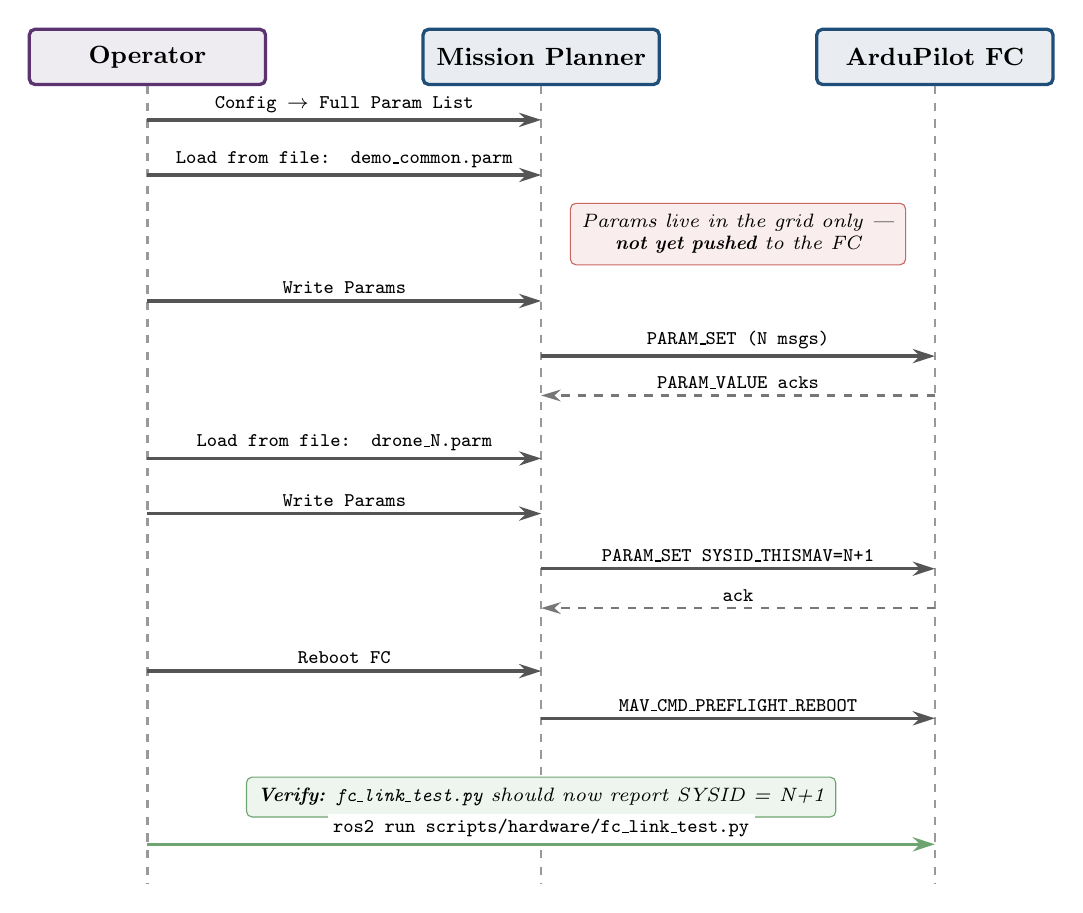
\begin{tikzpicture}[x=1cm, y=1cm]
  % --- Actor heads ---
  \node[sdactorops] (op) at (0, 0) {Operator};
  \node[sdactor]    (mp) at (5, 0) {Mission Planner};
  \node[sdactor]    (fc) at (10, 0) {ArduPilot FC};

  % --- Lifelines ---
  \def\bottom{-10.5}
  \draw[lifeline] (op) -- (0, \bottom);
  \draw[lifeline] (mp) -- (5, \bottom);
  \draw[lifeline] (fc) -- (10, \bottom);

  % --- Messages ---
  \draw[sdmsg] (0, -0.8) -- (5, -0.8) node[sdlab, midway, above]{Config $\to$ Full Param List};
  \draw[sdmsg] (0, -1.5) -- (5, -1.5) node[sdlab, midway, above]{Load from file: demo\_common.parm};

  % Note 1
  \node[notebox, anchor=center] at (7.5, -2.25)
    {Params live in the grid only ---\\\textbf{not yet pushed} to the FC};

  \draw[sdmsg] (0, -3.1) -- (5, -3.1) node[sdlab, midway, above]{\bfseries Write Params};
  \draw[sdmsg] (5, -3.8) -- (10, -3.8) node[sdlab, midway, above]{PARAM\_SET (N msgs)};
  \draw[sdret] (10, -4.3) -- (5, -4.3) node[sdlab, midway, above]{PARAM\_VALUE acks};

  \draw[sdmsg] (0, -5.1) -- (5, -5.1) node[sdlab, midway, above]{Load from file: drone\_N.parm};
  \draw[sdmsg] (0, -5.8) -- (5, -5.8) node[sdlab, midway, above]{\bfseries Write Params};
  \draw[sdmsg] (5, -6.5) -- (10, -6.5) node[sdlab, midway, above]{PARAM\_SET SYSID\_THISMAV=N+1};
  \draw[sdret] (10, -7.0) -- (5, -7.0) node[sdlab, midway, above]{ack};

  \draw[sdmsg] (0, -7.8) -- (5, -7.8) node[sdlab, midway, above]{Reboot FC};
  \draw[sdmsg] (5, -8.4) -- (10, -8.4) node[sdlab, midway, above]{MAV\_CMD\_PREFLIGHT\_REBOOT};

  % Verify note
  \node[notebox, anchor=center, draw=accentgreen!70, fill=accentgreen!8] at (5, -9.4)
    {\textbf{Verify:} \texttt{fc\_link\_test.py} should now report SYSID = N+1};
  \draw[sdmsg, draw=accentgreen!70] (0, -10.0) -- (10, -10.0)
    node[sdlab, midway, above]{ros2 run scripts/hardware/fc\_link\_test.py};

\end{tikzpicture}
\end{center}

\vspace{0.5em}

\begin{tcolorbox}[colback=bggrey, colframe=warnred, arc=2pt, boxrule=0.5pt,
                  title={\small\bfseries Gotcha}, fonttitle=\color{warnred}]
\textbf{``Load from file''} populates the parameter grid only --- it does \emph{not} push
to the FC. The \textbf{Write Params} button is what actually transmits. QGroundControl
combines the two; Mission Planner does not. Skipping ``Write Params'' is the most common
cause of a drone arming with unchanged defaults after what looked like a clean
parameter load.
\end{tcolorbox}

\newpage

% =================================================================
% §5 — Sequence: Arm + takeoff
% =================================================================
\section{Sequence: arm and takeoff via the swarm services}

What happens when the operator types
\texttt{ros2 service call /swarm/takeoff}. Note the parallel safety-pilot
lane --- their RC switch position is monitored throughout but does not
appear as a message; the FC handles RC override internally.

\vspace{0.6em}
\begin{center}
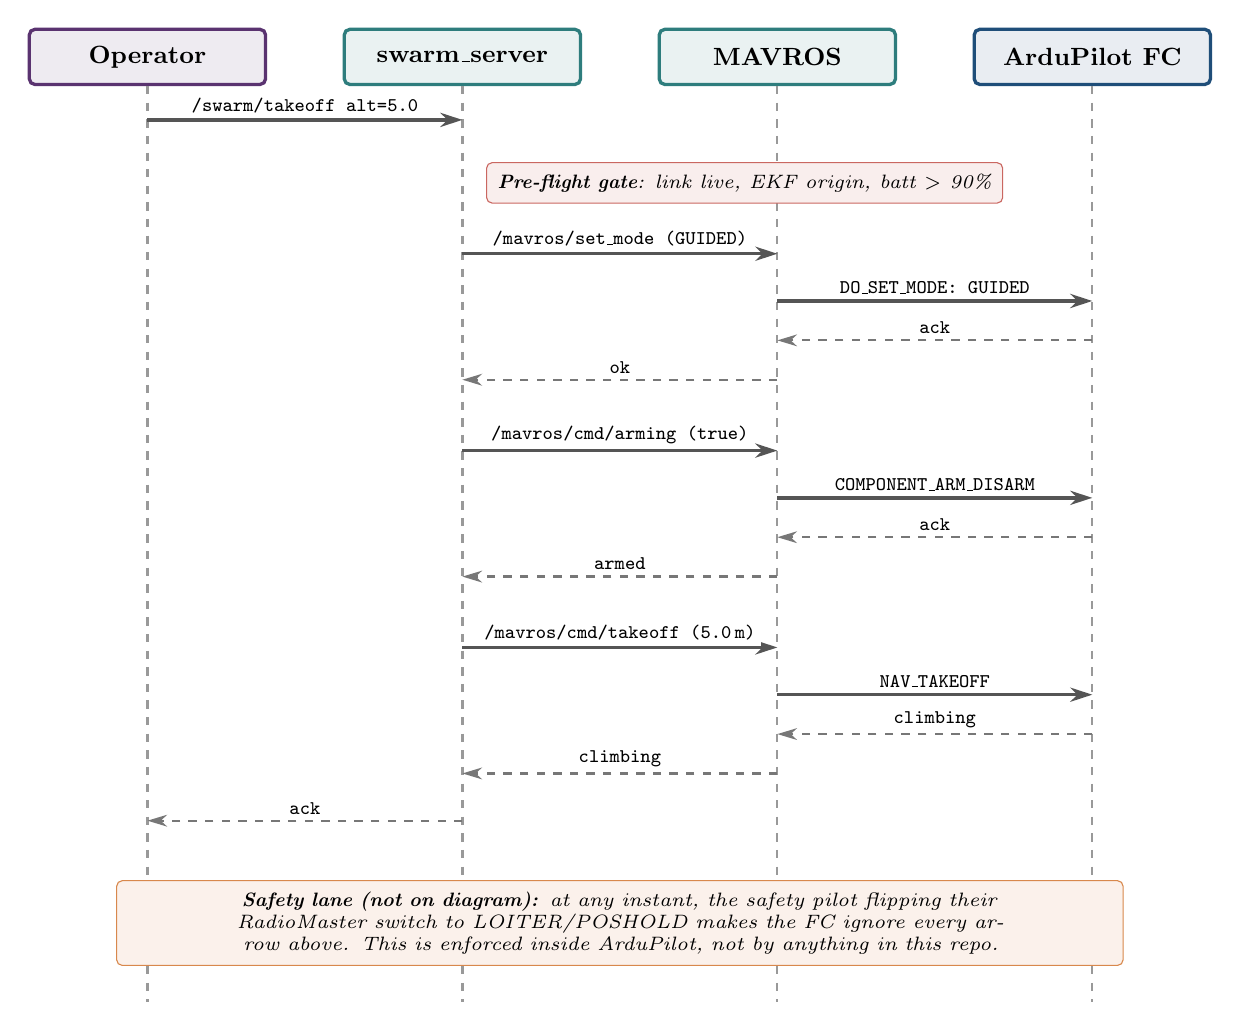
\begin{tikzpicture}[x=1cm, y=1cm]
  % --- Actors ---
  \node[sdactorops]  (op) at (0,  0) {Operator};
  \node[sdactorlight](sw) at (4,  0) {swarm\_server};
  \node[sdactorlight](mr) at (8,  0) {MAVROS};
  \node[sdactor]     (fc) at (12, 0) {ArduPilot FC};

  \def\bottom{-12.0}
  \draw[lifeline] (op) -- (0,  \bottom);
  \draw[lifeline] (sw) -- (4,  \bottom);
  \draw[lifeline] (mr) -- (8,  \bottom);
  \draw[lifeline] (fc) -- (12, \bottom);

  % --- Operator → swarm_server ---
  \draw[sdmsg] (0, -0.8) -- (4, -0.8) node[sdlab, midway, above]{/swarm/takeoff alt=5.0};

  % Pre-flight gate note
  \node[notebox, anchor=west] at (4.3, -1.6)
    {\textbf{Pre-flight gate}: link live, EKF origin, batt $>$ 90\%};

  % --- set_mode chain ---
  \draw[sdmsg] (4, -2.5) -- (8, -2.5)  node[sdlab, midway, above]{/mavros/set\_mode (GUIDED)};
  \draw[sdmsg] (8, -3.1) -- (12, -3.1) node[sdlab, midway, above]{DO\_SET\_MODE: GUIDED};
  \draw[sdret] (12, -3.6) -- (8, -3.6) node[sdlab, midway, above]{ack};
  \draw[sdret] (8, -4.1) -- (4, -4.1)  node[sdlab, midway, above]{ok};

  % --- arming chain ---
  \draw[sdmsg] (4, -5.0) -- (8, -5.0)  node[sdlab, midway, above]{/mavros/cmd/arming (true)};
  \draw[sdmsg] (8, -5.6) -- (12, -5.6) node[sdlab, midway, above]{COMPONENT\_ARM\_DISARM};
  \draw[sdret] (12, -6.1) -- (8, -6.1) node[sdlab, midway, above]{ack};
  \draw[sdret] (8, -6.6) -- (4, -6.6)  node[sdlab, midway, above]{armed};

  % --- takeoff chain ---
  \draw[sdmsg] (4, -7.5) -- (8, -7.5)  node[sdlab, midway, above]{/mavros/cmd/takeoff (5.0\,m)};
  \draw[sdmsg] (8, -8.1) -- (12, -8.1) node[sdlab, midway, above]{NAV\_TAKEOFF};
  \draw[sdret] (12, -8.6) -- (8, -8.6) node[sdlab, midway, above]{climbing};
  \draw[sdret] (8, -9.1) -- (4, -9.1)  node[sdlab, midway, above]{climbing};
  \draw[sdret] (4, -9.7) -- (0, -9.7)  node[sdlab, midway, above]{ack};

  % Safety lane note
  \node[notebox, anchor=center, draw=rcorange!70, fill=rcorange!8,
        text width=12.5cm] at (6, -11.0)
    {\textbf{Safety lane (not on diagram):} at any instant, the safety pilot flipping their
     RadioMaster switch to LOITER/POSHOLD makes the FC ignore every arrow above.
     This is enforced inside ArduPilot, not by anything in this repo.};

\end{tikzpicture}
\end{center}

\vspace{0.5em}

\begin{tcolorbox}[colback=lightaccent, colframe=fcblue, arc=2pt, boxrule=0.4pt,
                  title={\small\bfseries Safety lane}, fonttitle=\color{fcblue}]
The dim lane on the right is the safety pilot's RC. At any point the safety pilot can
flip a mode switch to \textbf{LOITER} or \textbf{POSHOLD} and the FC ignores all
subsequent \texttt{swarm\_server} commands until they switch back to GUIDED. This is
enforced by ArduPilot, not by anything in this repository --- it is the layer below all
of these arrows.
\end{tcolorbox}

\newpage

% =================================================================
% §6 — Sequence: Leader-follow
% =================================================================
\section{Sequence: leader-follow, with watchdog}

The defining behaviour of Phase~2.5b. Leader pose flows over the
Cyclone DDS LAN; each follower's \texttt{swarm\_server} computes a slot
offset and feeds setpoints into MAVROS. A watchdog guards the leader
pose against link drop.

\vspace{0.6em}
\begin{center}
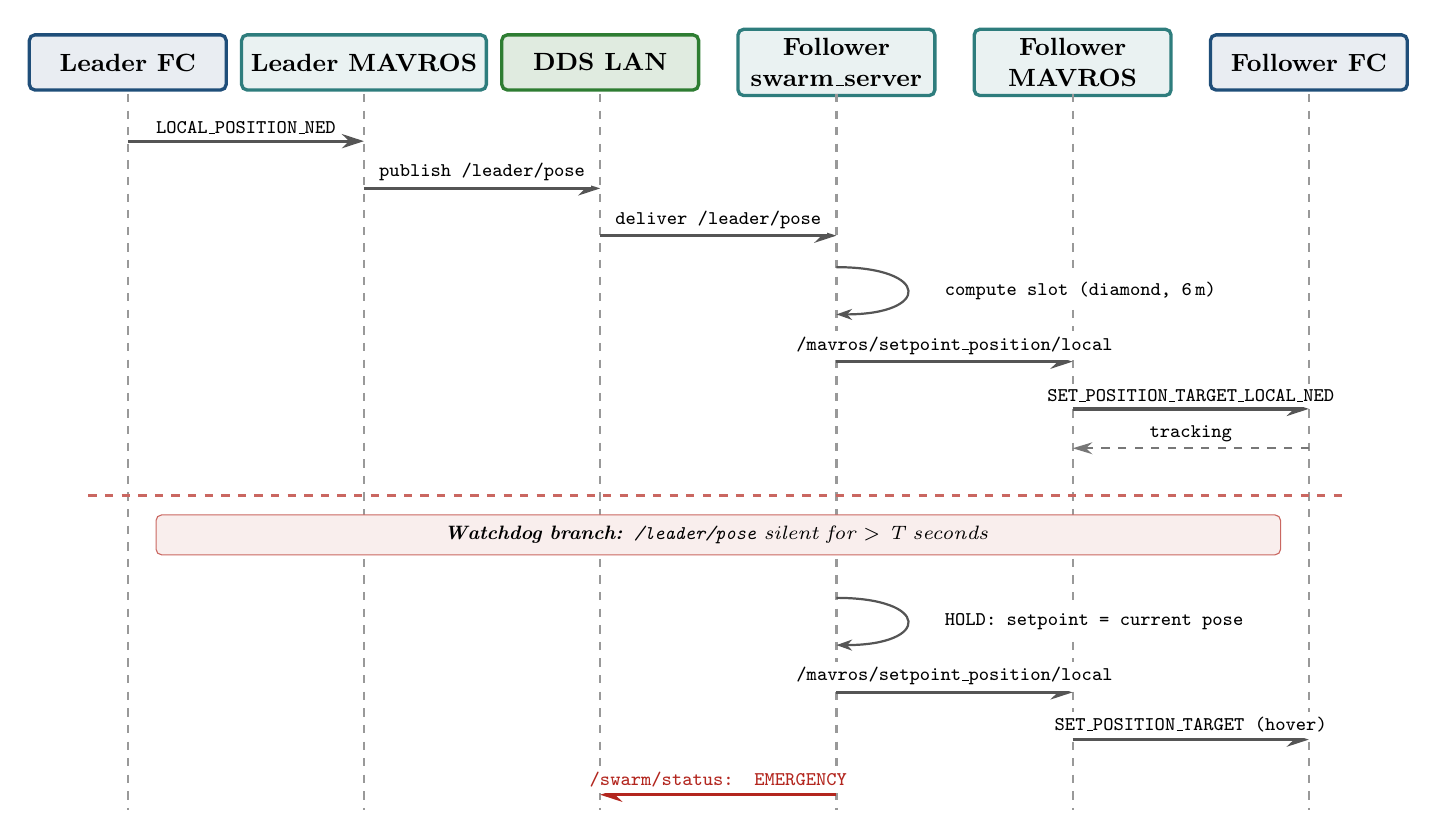
\begin{tikzpicture}[x=1cm, y=1cm]
  % --- Actors (6 across) ---
  \node[sdactor,      minimum width=2.5cm] (lfc) at (0,  0)  {Leader FC};
  \node[sdactorlight, minimum width=2.5cm] (lmr) at (3,  0)  {Leader MAVROS};
  \node[sdactor,      minimum width=2.5cm, fill=accentgreen!15, draw=accentgreen]
                                           (dds) at (6,  0)  {DDS LAN};
  \node[sdactorlight, minimum width=2.5cm] (fsw) at (9,  0)  {Follower\\swarm\_server};
  \node[sdactorlight, minimum width=2.5cm] (fmr) at (12, 0)  {Follower\\MAVROS};
  \node[sdactor,      minimum width=2.5cm] (ffc) at (15, 0)  {Follower FC};

  \def\bottom{-9.5}
  \foreach \x in {0,3,6,9,12,15}{\draw[lifeline] (\x, -0.4) -- (\x, \bottom);}

  % --- Nominal flow ---
  \draw[sdmsg] (0, -1.0) -- (3, -1.0)   node[sdlab, midway, above]{LOCAL\_POSITION\_NED};
  \draw[sdmsg] (3, -1.6) -- (6, -1.6)   node[sdlab, midway, above]{publish /leader/pose};
  \draw[sdmsg] (6, -2.2) -- (9, -2.2)   node[sdlab, midway, above]{deliver /leader/pose};

  % Self-call: slot computation
  \draw[sdself] (9, -2.6) .. controls (10.2, -2.6) and (10.2, -3.2) .. (9, -3.2);
  \node[sdlab, anchor=west] at (10.3, -2.9) {compute slot (diamond, 6\,m)};

  \draw[sdmsg] (9,  -3.8) -- (12, -3.8) node[sdlab, midway, above]{/mavros/setpoint\_position/local};
  \draw[sdmsg] (12, -4.4) -- (15, -4.4) node[sdlab, midway, above]{SET\_POSITION\_TARGET\_LOCAL\_NED};
  \draw[sdret] (15, -4.9) -- (12, -4.9) node[sdlab, midway, above]{tracking};

  % Watchdog branch separator
  \draw[draw=warnred!70, very thick, dashed] (-0.5, -5.5) -- (15.5, -5.5);
  \node[anchor=west, font=\small\bfseries\color{warnred}] at (-0.4, -5.5) {};
  \node[notebox, anchor=center, text width=14cm] at (7.5, -6.0)
    {\textbf{Watchdog branch:} \texttt{/leader/pose} silent for $>$ T seconds};

  % Watchdog flow
  \draw[sdself] (9, -6.8) .. controls (10.2, -6.8) and (10.2, -7.4) .. (9, -7.4);
  \node[sdlab, anchor=west] at (10.3, -7.1) {HOLD: setpoint = current pose};

  \draw[sdmsg] (9,  -8.0) -- (12, -8.0) node[sdlab, midway, above]{/mavros/setpoint\_position/local};
  \draw[sdmsg] (12, -8.6) -- (15, -8.6) node[sdlab, midway, above]{SET\_POSITION\_TARGET (hover)};
  \draw[sdmsg, draw=warnred] (9, -9.3) -- (6, -9.3)
        node[sdlab, midway, above]{\color{warnred}/swarm/status: EMERGENCY};

\end{tikzpicture}
\end{center}

\vspace{0.5em}

\noindent\textbf{Acceptance gates} (from \texttt{PLAN.md}~\S D, Phase~2.5b): mean horizontal
formation error \textless~2\,m per follower over $\geq$~60\,s of leader motion;
watchdog demonstrably holds on a simulated link drop; coordinated land; recorded as
\texttt{accept/demo\_leaderfollow.mcap}.

\newpage

% =================================================================
% §7 — Network topology
% =================================================================
\section{Swarm network topology}

Five drones on a shared WiFi LAN. Cyclone DDS provides the inter-drone
ROS 2 fabric; Zenoh selectively forwards a small subset of topics out
to the operator (ADR~0004).

\vspace{0.6em}
\begin{center}
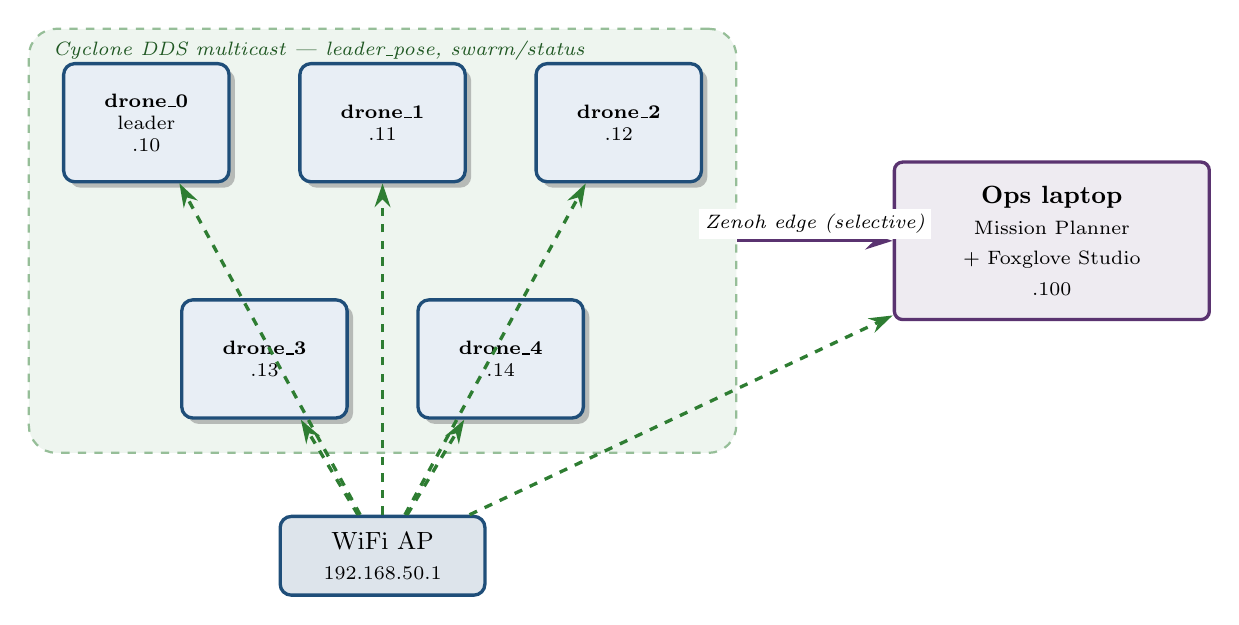
\begin{tikzpicture}[x=1cm, y=1cm]
  % Drones laid out in a 2x3 grid on the left
  \node[drone] (d0) at (0,   3) {\textbf{drone\_0}\\leader\\\scriptsize .10};
  \node[drone] (d1) at (3,   3) {\textbf{drone\_1}\\\scriptsize .11};
  \node[drone] (d2) at (6,   3) {\textbf{drone\_2}\\\scriptsize .12};
  \node[drone] (d3) at (1.5, 0) {\textbf{drone\_3}\\\scriptsize .13};
  \node[drone] (d4) at (4.5, 0) {\textbf{drone\_4}\\\scriptsize .14};

  % WiFi AP centred below the drones
  \node[draw=fcblue, very thick, rounded corners, fill=fcblue!15, font=\small,
        minimum width=2.6cm, minimum height=1cm, align=center] (ap) at (3, -2.5)
        {WiFi AP\\\scriptsize 192.168.50.1};

  % Operator laptop far to the right
  \node[gcsbox, minimum width=4cm, minimum height=2cm, align=center] (laptop) at (11.5, 1.5)
       {\textbf{Ops laptop}\\\scriptsize Mission Planner\\\scriptsize + Foxglove Studio\\\scriptsize .100};

  % DDS multicast cloud around the 5 drones only
  \begin{scope}[on background layer]
    \node[draw=accentgreen!50, fill=accentgreen!8, thick, dashed,
          rounded corners=10pt, fit=(d0)(d1)(d2)(d3)(d4),
          inner sep=12pt] (ddscloud) {};
  \end{scope}
  \node[anchor=north west, font=\scriptsize\itshape\color{accentgreen!70!black}]
    at ([xshift=0.2cm, yshift=-0.05cm]ddscloud.north west)
    {Cyclone DDS multicast --- leader\_pose, swarm/status};

  % WiFi links AP to drones and laptop
  \foreach \d in {d0,d1,d2,d3,d4}{\draw[link, draw=accentgreen, dashed] (ap) -- (\d);}
  \draw[link, draw=accentgreen, dashed] (ap) -- (laptop);

  % Zenoh edge from cloud (east) to laptop (west) — clearly outside the cloud
  \draw[->, very thick, >={Stealth[length=3.5mm,width=2.2mm]}, draw=gcspurple]
        (ddscloud.east) -- node[linklabel, above]{Zenoh edge (selective)} (laptop.west);

\end{tikzpicture}
\end{center}

\vspace{0.6em}

\begin{center}
\small
\begin{tabularx}{0.95\textwidth}{@{}llX@{}}
\toprule
\textbf{Address} & \textbf{Host} & \textbf{Role} \\
\midrule
\texttt{192.168.50.10} & \texttt{drone\_0} & Leader; \texttt{SYSID\_THISMAV}=1; manually flown on RC; publishes \texttt{/leader/pose} \\
\texttt{192.168.50.11--14} & \texttt{drone\_1..4} & Followers; \texttt{SYSID\_THISMAV}=2..5; autonomous GUIDED \\
\texttt{192.168.50.100} & ops laptop & Mission Planner + Foxglove Studio; runs \texttt{ros2 service call /swarm/...} \\
\bottomrule
\end{tabularx}
\end{center}

\noindent\textbf{Why this split.} Cyclone DDS is great inside the LAN (multicast, low
latency, but chatty on discovery). Zenoh on the edge filters the firehose down to just
the topics the operator actually needs --- formation pose, status, telemetry summary
--- avoiding the operator laptop being saturated with intra-swarm chatter
(\texttt{PLAN.md}~\S A, ADR~0004).

\newpage

% =================================================================
% §8 — Three deployment modes side by side
% =================================================================
\section{The three deployment modes, side by side}

Same architecture, different ``FC'' box. The MAVROS / swarm\_server /
Foxglove layer above is identical across all three.

\vspace{0.6em}

% A reusable column: builds one of the three stacks at the current scope origin.
% Args: #1=title, #2=operator label, #3=foxglove label, #4=swarm label,
%       #5=mavros label, #6=FC label, #7=link label between mavros & FC, #8=footer.
\newcommand{\modeColumn}[8]{%
\begin{minipage}[t]{0.32\textwidth}
\centering
{\small\bfseries\color{fcblue} #1}\\[0.3em]
\begin{tikzpicture}[x=1cm, y=1cm, every node/.style={font=\scriptsize}]
  \node[gcsbox, minimum width=4.6cm, minimum height=0.8cm] (op) at (0, 0)    {#2};
  \node[swcomp, minimum width=4.6cm, minimum height=0.7cm] (fx) at (0, -1.0) {#3};
  \node[swcomp, minimum width=4.6cm, minimum height=0.7cm] (sw) at (0, -2.0) {#4};
  \node[swcomp, minimum width=4.6cm, minimum height=0.7cm] (mr) at (0, -3.0) {#5};
  \node[fcbox,  minimum width=4.6cm, minimum height=1.2cm] (fc) at (0, -4.4) {#6};
  \draw[link] (op) -- (fx);
  \draw[link] (fx) -- (sw);
  \draw[link] (sw) -- (mr);
  \draw[link] (mr) -- node[linklabel, right]{#7} (fc);
\end{tikzpicture}\\[0.3em]
{\scriptsize\itshape\color{gray!70} #8}
\end{minipage}}

\begin{center}
\modeColumn
  {compose.dev.yaml}
  {Operator (host)}
  {foxglove\_bridge}
  {swarm\_server}
  {MAVROS}
  {\texttt{arducopter} (SITL)\\\scriptsize TCP/UDP endpoint}
  {MAVLink/UDP}
  {single drone, no hardware --- daily dev loop}
\hfill
\modeColumn
  {compose.swarm.yaml}
  {Operator (host)}
  {foxglove\_bridge (leader)}
  {5$\times$ swarm\_server}
  {5$\times$ MAVROS}
  {5$\times$ \texttt{arducopter}\\\scriptsize via \texttt{sitl\_launcher.py}}
  {5 endpoints}
  {five-drone SITL --- CI \& acceptance}
\hfill
\modeColumn
  {compose.hw / .demo.yaml}
  {Operator (ops laptop)}
  {foxglove\_bridge (per-drone)}
  {swarm\_server (per-drone)}
  {MAVROS (per-drone)}
  {\textbf{real FC}\\\scriptsize \texttt{serial:///dev/ttyTHS1}}
  {UART}
  {real airframe(s) --- Phase 2.5b demo \& Phase 6 HIL}
\end{center}

\vspace{0.8em}

\begin{tcolorbox}[colback=lightaccent, colframe=fcblue, arc=2pt, boxrule=0.4pt]
\textbf{The portability claim, made concrete.} The MAVROS / swarm\_server /
foxglove\_bridge blocks above the FC box are \emph{identical} across all three
columns. They speak MAVLink to whatever happens to be sitting in the FC box ---
a simulated \texttt{arducopter} process, five of them, or your real Pixhawk over a
UART. This is why a green \texttt{make leaderfollow-smoke} in SITL is a real
prerequisite for the bench flight: the same code runs in both.
\end{tcolorbox}

\newpage

% =================================================================
% §9 — Field setup
% =================================================================
\section{Field setup: who stands where (Phase 2.5b)}

Top-down view of the operating area during the leader-follow demo.
Roles per \texttt{docs/runbooks/first\_flight.md}~\S1.

\vspace{0.6em}
\begin{center}
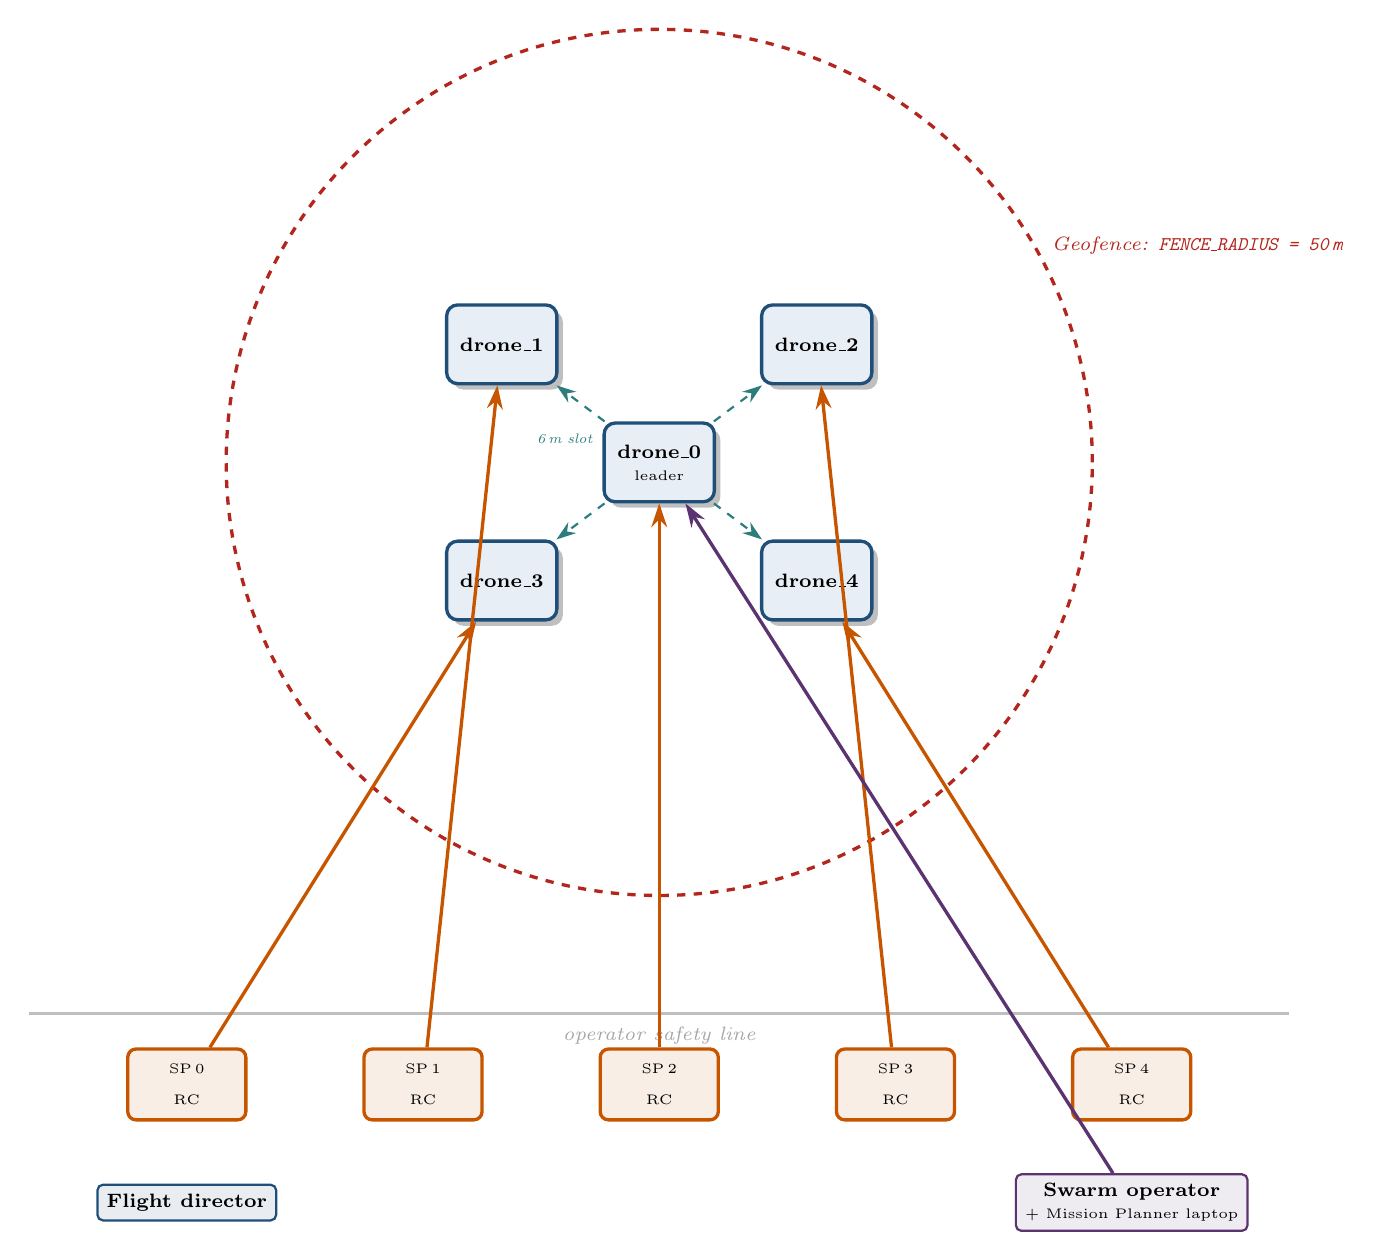
\begin{tikzpicture}[node distance=1cm]
  % --- Geofence circle ---
  \draw[draw=warnred, very thick, dashed] (0,0) circle (5.5cm);
  \node[font=\scriptsize\itshape, text=warnred, anchor=west]
    at ([xshift=0.1cm]30:5.5cm) {Geofence: \texttt{FENCE\_RADIUS = 50\,m}};

  % --- Drones in diamond formation ---
  \node[drone, minimum width=1.4cm, minimum height=1.0cm] (ld) at (0,0)   {\textbf{drone\_0}\\\tiny leader};
  \node[drone, minimum width=1.4cm, minimum height=1.0cm] (f1) at (-2,1.5)  {\textbf{drone\_1}};
  \node[drone, minimum width=1.4cm, minimum height=1.0cm] (f2) at (2,1.5)   {\textbf{drone\_2}};
  \node[drone, minimum width=1.4cm, minimum height=1.0cm] (f3) at (-2,-1.5) {\textbf{drone\_3}};
  \node[drone, minimum width=1.4cm, minimum height=1.0cm] (f4) at (2,-1.5)  {\textbf{drone\_4}};

  % Formation links
  \foreach \f in {f1,f2,f3,f4} {
    \draw[faintlink, draw=jetsonteal] (ld) -- (\f);
  }
  \node[font=\tiny\itshape\color{jetsonteal}] at (-1.2,0.3) {6\,m slot};

  % --- Operating positions (outside the cone-of-fire, behind a line) ---
  \draw[draw=gray!50, very thick] (-8,-7) -- (8,-7);
  \node[font=\scriptsize\itshape\color{gray!70}, anchor=north] at (0,-7.05) {operator safety line};

  \node[rcbox, minimum width=1.5cm, minimum height=0.9cm] (sp0) at (-6,-7.9) {\tiny SP\,0\\\tiny RC};
  \node[rcbox, minimum width=1.5cm, minimum height=0.9cm] (sp1) at (-3,-7.9) {\tiny SP\,1\\\tiny RC};
  \node[rcbox, minimum width=1.5cm, minimum height=0.9cm] (sp2) at (0,-7.9)  {\tiny SP\,2\\\tiny RC};
  \node[rcbox, minimum width=1.5cm, minimum height=0.9cm] (sp3) at (3,-7.9)  {\tiny SP\,3\\\tiny RC};
  \node[rcbox, minimum width=1.5cm, minimum height=0.9cm] (sp4) at (6,-7.9)  {\tiny SP\,4\\\tiny RC};

  \node[font=\scriptsize, draw=fcblue, fill=fcblue!10, thick, rounded corners=2pt, align=center]
    (fd) at (-6,-9.4) {\bfseries Flight director};
  \node[font=\scriptsize, draw=gcspurple, fill=gcspurple!10, thick, rounded corners=2pt, align=center]
    (swop) at (6,-9.4) {\bfseries Swarm operator\\\tiny + Mission Planner laptop};

  % Lines of authority/visibility
  \draw[link, draw=rcorange] (sp0) -- (f3);
  \draw[link, draw=rcorange] (sp1) -- (f1);
  \draw[link, draw=rcorange] (sp2) -- (ld);
  \draw[link, draw=rcorange] (sp3) -- (f2);
  \draw[link, draw=rcorange] (sp4) -- (f4);
  \draw[link, draw=gcspurple] (swop) -- (ld);

\end{tikzpicture}
\end{center}

\vspace{0.5em}

\begin{center}
\small
\begin{tabularx}{0.95\textwidth}{@{}lcX@{}}
\toprule
\textbf{Role} & \textbf{Count} & \textbf{What they hold / where they look} \\
\midrule
Flight director & 1 & No equipment --- calls the sequence, owns go/no-go, calls aborts. \\
Safety pilot (SP) & \textbf{1 per drone} & Their drone's RadioMaster TX; mode switch ready. \\
Swarm operator & 1 & Ops laptop: Mission Planner (MAVLink monitor) + Foxglove (formation view); runs the \texttt{/swarm/*} service calls. \\
\bottomrule
\end{tabularx}
\end{center}

\photoplaceholder{15}{5.0}{Suggested shot: the field with drones laid out in the
diamond, safety pilots behind the safety line each holding their RadioMaster,
operator at the laptop in the foreground. Save to
\texttt{images/field\_phase\_2\_5b.jpg}.}

\newpage

% =================================================================
% §10 — Authority hierarchy & failsafe waterfall
% =================================================================
\section{Authority hierarchy and the failsafe waterfall}\label{sec:authority}

Who wins when two channels disagree, and what the firmware does on its
own when a channel disappears.

\vspace{0.6em}

\noindent\textbf{Authority pyramid} --- ArduPilot resolves conflicting commands top-down:

\begin{center}
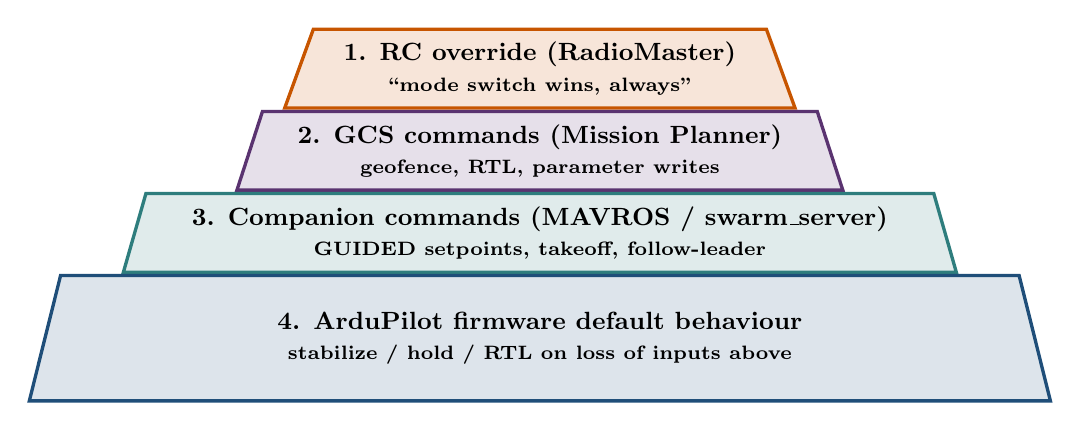
\begin{tikzpicture}[node distance=0.0cm]
  \node[draw=rcorange, very thick, fill=rcorange!15, trapezium, trapezium left angle=70, trapezium right angle=70,
        minimum width=4cm, minimum height=1cm, align=center, font=\small\bfseries]
        (l1) {1. RC override (RadioMaster)\\\scriptsize ``mode switch wins, always''};
  \node[draw=gcspurple, very thick, fill=gcspurple!15, trapezium, trapezium left angle=72, trapezium right angle=72,
        minimum width=7cm, minimum height=1cm, align=center, font=\small\bfseries, below=0cm of l1]
        (l2) {2. GCS commands (Mission Planner)\\\scriptsize geofence, RTL, parameter writes};
  \node[draw=jetsonteal, very thick, fill=jetsonteal!15, trapezium, trapezium left angle=74, trapezium right angle=74,
        minimum width=10cm, minimum height=1cm, align=center, font=\small\bfseries, below=0cm of l2]
        (l3) {3. Companion commands (MAVROS / swarm\_server)\\\scriptsize GUIDED setpoints, takeoff, follow-leader};
  \node[draw=fcblue, very thick, fill=fcblue!15, trapezium, trapezium left angle=76, trapezium right angle=76,
        minimum width=13cm, minimum height=1cm, align=center, font=\small\bfseries, below=0cm of l3]
        (l4) {4. ArduPilot firmware default behaviour\\\scriptsize stabilize / hold / RTL on loss of inputs above};
\end{tikzpicture}
\end{center}

\vspace{0.8em}

\noindent\textbf{Failsafe waterfall} --- what trips, in what order, when something goes wrong:

\begin{center}
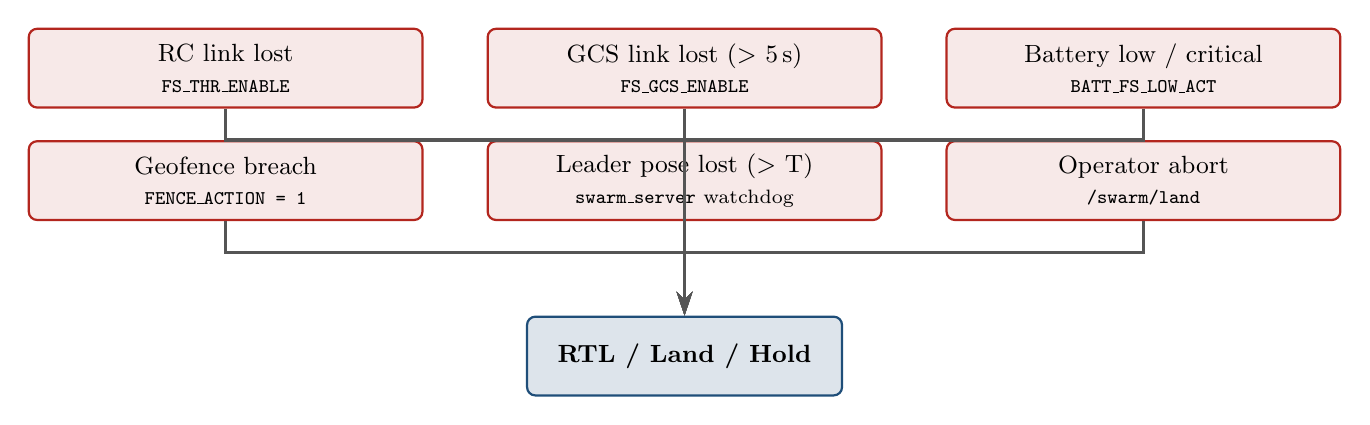
\begin{tikzpicture}[node distance=0.4cm and 0.8cm, every node/.style={font=\small}]
  \node[draw=warnred, fill=warnred!10, thick, rounded corners=3pt, minimum width=5cm, minimum height=1cm, align=center]
        (rc) {RC link lost\\\scriptsize\texttt{FS\_THR\_ENABLE}};
  \node[draw=warnred, fill=warnred!10, thick, rounded corners=3pt, minimum width=5cm, minimum height=1cm, align=center, right=of rc]
        (gcs) {GCS link lost ($>$ 5\,s)\\\scriptsize\texttt{FS\_GCS\_ENABLE}};
  \node[draw=warnred, fill=warnred!10, thick, rounded corners=3pt, minimum width=5cm, minimum height=1cm, align=center, right=of gcs]
        (batt) {Battery low / critical\\\scriptsize\texttt{BATT\_FS\_LOW\_ACT}};

  \node[draw=warnred, fill=warnred!10, thick, rounded corners=3pt, minimum width=5cm, minimum height=1cm, align=center, below=of rc]
        (fence) {Geofence breach\\\scriptsize\texttt{FENCE\_ACTION = 1}};
  \node[draw=warnred, fill=warnred!10, thick, rounded corners=3pt, minimum width=5cm, minimum height=1cm, align=center, below=of gcs]
        (leader) {Leader pose lost ($>$ T)\\\scriptsize \texttt{swarm\_server} watchdog};
  \node[draw=warnred, fill=warnred!10, thick, rounded corners=3pt, minimum width=5cm, minimum height=1cm, align=center, below=of batt]
        (operator) {Operator abort\\\scriptsize \texttt{/swarm/land}};

  \node[draw=fcblue, fill=fcblue!15, thick, rounded corners=3pt, minimum width=4cm, minimum height=1cm, align=center,
        below=1.2cm of leader, font=\small\bfseries]
        (rtl) {RTL / Land / Hold};

  \draw[link] (rc) |- ([yshift=-0.4cm]rc.south) -| (rtl.north);
  \draw[link] (gcs) |- ([yshift=-0.4cm]gcs.south) -| (rtl.north);
  \draw[link] (batt) |- ([yshift=-0.4cm]batt.south) -| (rtl.north);
  \draw[link] (fence) |- ([yshift=-0.4cm]fence.south) -| (rtl.north);
  \draw[link] (leader) -- (rtl.north);
  \draw[link] (operator) |- ([yshift=-0.4cm]operator.south) -| (rtl.north);
\end{tikzpicture}
\end{center}

\vspace{0.8em}

\begin{tcolorbox}[colback=bggrey, colframe=linegrey!50, arc=2pt, boxrule=0.4pt,
                  title={\small\bfseries One distinction worth keeping straight}, fonttitle=\color{fcblue}]
The first four failsafes are \emph{firmware-level} --- they fire inside ArduPilot
regardless of the state of the Jetson, MAVROS, or even whether the operator is
paying attention. The fifth, \emph{leader pose lost}, is the only swarm-specific
failsafe and lives in \texttt{swarm\_server}; it holds followers in place rather
than triggering RTL, because RTL on five drones at once is its own kind of
incident.
\end{tcolorbox}

\newpage

% =================================================================
% §11 — Repo pointers
% =================================================================
\section{Where it all lives in the repo}

\small
\begin{tabularx}{\textwidth}{@{}llX@{}}
\toprule
\textbf{What you saw} & \textbf{Section} & \textbf{Where in the repo} \\
\midrule
Stack picks & §1 & \texttt{PLAN.md}~\S A (decision record) \\
MAVROS choice & §3 & \texttt{docs/adr/0002-mavros-over-ap-dds-for-now.md} \\
DDS + Zenoh split & §3, §7 & \texttt{docs/adr/0004-cyclone-dds-plus-zenoh-edge.md} \\
SITL simulator path & §8 & \texttt{docs/adr/0003-gazebo-harmonic-ardupilot-gz.md} \\
Leader-follow demo plan & §6, §9 & \texttt{docs/adr/0008-leader-follow-demo-integration.md} \\
Single-drone dev compose & §8 & \texttt{docker/compose.dev.yaml} \\
Five-drone SITL compose & §8 & \texttt{docker/compose.swarm.yaml} \\
Hardware composes (Phase 2.5b) & §8 & \texttt{docker/compose.hw.yaml}, \texttt{compose.demo.yaml} \\
Param load procedure & §4 & \texttt{config/ardupilot\_params/README.md} \\
Per-drone parameter files & §4 & \texttt{config/ardupilot\_params/demo\_common.parm}, \texttt{drone\_N.parm} \\
First-flight checklist & §9, §10 & \texttt{docs/runbooks/first\_flight.md} \\
Day-to-day operator runbook & §7, §9 & \texttt{docs/runbooks/jetson\_swarm\_operations.md} \\
swarm\_server services & §5, §6 & \texttt{ros2\_ws/src/swarm\_server/} \\
Bringup scripts & §9 & \texttt{scripts/bringup/demo\_swarm.sh} \\
FC link verification & §4 & \texttt{scripts/hardware/fc\_link\_test.py} \\
Phase status (live) & all & \texttt{WORKFLOW.md} \\
\bottomrule
\end{tabularx}

\vspace{1em}

\begin{tcolorbox}[colback=lightaccent, colframe=fcblue, arc=2pt, boxrule=0.4pt,
                  title={\small\bfseries Reading order if you want to dig deeper},
                  fonttitle=\color{fcblue}]
\begin{enumerate}[leftmargin=*, itemsep=0.2em]
  \item \texttt{PLAN.md} --- the canonical stack picks and roadmap.
  \item \texttt{docs/architecture/overview.md} --- ADR index in suggested reading order.
  \item ADRs 0001--0008 --- one decision each, with the rationale.
  \item \texttt{docs/runbooks/first\_flight.md} --- the hardware demo gate \& procedure.
\end{enumerate}
\end{tcolorbox}

\vfill

\begin{center}
\small\itshape
End of document. To swap a placeholder for an actual photo, drop a JPG into
\texttt{images/} and uncomment the matching \textbackslash{}includegraphics line
in the source.
\end{center}

\end{document}
